\documentclass[10pt,a4paper]{book}
\usepackage[utf8]{inputenc}
\usepackage[french]{babel}
\usepackage[T1]{fontenc}
\usepackage{amsmath}
\usepackage{amsfonts}
\usepackage{amssymb}
\usepackage{geometry}
\usepackage{graphicx}
\usepackage{wrapfig}
\usepackage{subcaption}
\geometry{top=4cm, bottom=4cm, left=2cm, right=2cm}
\author{ Antoine Robin}
\newcommand{\croisade}{Croisade Callidane }
\newcommand{\zone}{Tulea }
\newcommand{\secteur}{secteur Coronid }
\newcommand{\front}{front cyclopéen }
\title{Zone de guerre : \zone}
\begin{document}
\maketitle

\includegraphics[width=\textwidth]{aquila 2.png}
\tableofcontents
%12 ans de campagne pour cette croisade
\chapter{Introduction :  \croisade}
\section{Le \secteur}
Le \secteur est situé entre les segmentum Obsucurs et Ultima. Lourdement industrialisé lors de l'Hérésie d'Horus, il vit de violents combats entre les forces rebelles et loyalistes.

Après le siège de Terra et la mort d'Horus, les secteur tombé sous sa coupe furent progressivement repris par l'Imperium au cours des siècles suivant. Le \secteur revint dans le giron de l'Empereur au début du 32ème millénaire, les forces impériales s'emparant rapidement des planètes aux mains de seigneurs de guerre sans envergure.

Au cours des millénaires suivant, le secteur perdit à nouveau, cette fois progressivement, son contrôle sur ses régions périphériques : rebellions, oubli, abandon.... Au point qu'au 38ème millénaire, l'ensemble du secteur fut basculé dans le secteur Gothique, Port-Maw donnant son nom au nouveau sous-secteur. La proximité de l'œil de la terreur rend la région dangereuse : de nombreux pirates, pillards, renégats et traîtres rôdent facilement aux frontières de l'espace impérial. Le sous-secteur fut notamment attaqué par les forces du chaos lors de la 12ème croisade noire et la guerre gothique, lorsque les forces de l'ennemi tentèrent de neutraliser les puissantes installations portuaires.

\begin{wrapfigure}{l}{0.3\textwidth}
  \centering
  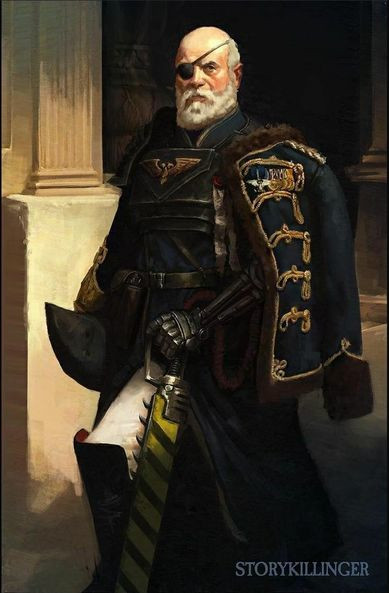
\includegraphics[width = 0.3\textwidth]{officer 3.jpg}
  \caption{Portrait officiel du maître de guerre Callidon}
\end{wrapfigure}

Au milieu du 41ème millénaire, la corruption commença à s'étendre depuis le monde de Baroda, un ancien monde-forge du mechanicus, lourdement pénalisé depuis sa trahison lors de la Grande Hérésie. Ses adeptes rejetèrent la dîme impériale, et bientôt, leurs vaisseaux explorateurs commencèrent à croiser l'espace voisin pour sécuriser des ressources, esclaves et matériaux. Ayant renversés leurs anciens maîtres du Mechanicus, les nouveaux seigneurs de Baroda, les maîtres ordinant révélèrent leur véritable allégeance, alors que des glyphes ignobles commencèrent à corrompre leurs créations, désormais mues par l'influence corruptrice du Warp.


Leurs sombres navires commencèrent à piller les régions voisines, propageant également leur culte immonde à de nombreux mondes des environs. Le temps que l'Imperium se rendre compte de la menace, la majeure partie des mondes oubliés de l'Imperium servaient, volontairement ou non les maîtres de Baroda.


La haute valeur stratégique de la région, ainsi que l'ampleur de la corruption qui se répandait aux frontières de l'espace impérial déclenchèrent une réaction importante, les hauts-seigneur de Terra décidant en 851M41 d'ordonner le lancement de la \croisade pour ramener ces mondes dans la lumière de l'Empereur. Pour mener cet effort, le maréchal Callidon fut nommé maître de guerre, et se vit confier de nombreuses troupes de l'astra militarum, de l'adeptus mechanicus, de la flotte impériale, mais aussi de l'adepta sororita et de l'adeptus astartes. Avec une telle concentration de forces à sa disposition, il entreprit de planifier l'opération d'envergure qui devait servir d'ouverture à a croisade : l'opération Defiance. 
\section{Opération Defiance}
%première partie de l'offensive impériale, visant à sécurisé le coeur du secteur
Cette opération connu de nombreuses itérations, toutes rejetées par le nouveau maître de guerre, qui n'appréciait pas la prudence de son état-major. Le plan final impliquait la sécurisation de plusieurs planètes impériales cibles de raids, et une offensive majeure vers les planètes ennemies, en particulier le monde-forteresse de Fellwatch devait être pris d'assaut, ainsi qu'une demi douzaine de monde plus secondaires, mais qui devaient servir de point d'appui à la croisade pour continuer.

La cible principale, Fellwatch fut assiégée par un puissant corps d'armée impérial, qui réalisa une offensive orbitale quelques dizaines d'heures après son transit hors du Warp. Après trois jours de sanglants combats, des space marines du chapitre des Carcharodons réussirent une percée sur le centre de commandement principal des forces hérétiques, massacrant l'hérémagos Kolstak et détruisant les communications des forces hérétiques. Cela brisa rapidement le moral des défenseurs, qui furent traqués par les forces impériales, même si des groupes de renégats continuèrent à mener des actions de guerrilla au cours des années suivantes.

Bedonov Tertius, un autre monde faisant partie des cibles de cette première phase, tomba après quelques semaines d'affrontements féroces, notamment au niveau du fort orbital \emph{Whisper of destruction}, qui fut abordé par plusieurs régiments de l'astra militarum après un engagement naval de deux jours, coûtant à l'escadre impérial le croiseur lourd \emph{Light of Cadia}. Une fois les défenses orbitales surclassées, les forces hérétiques sur place furent anéanties depuis l'orbite. La planète et ses installations orbitale servent maintenant de relai majeur pour la flotte de la croisade.

\begin{wrapfigure}{r}{0.3\textwidth}
  \centering
  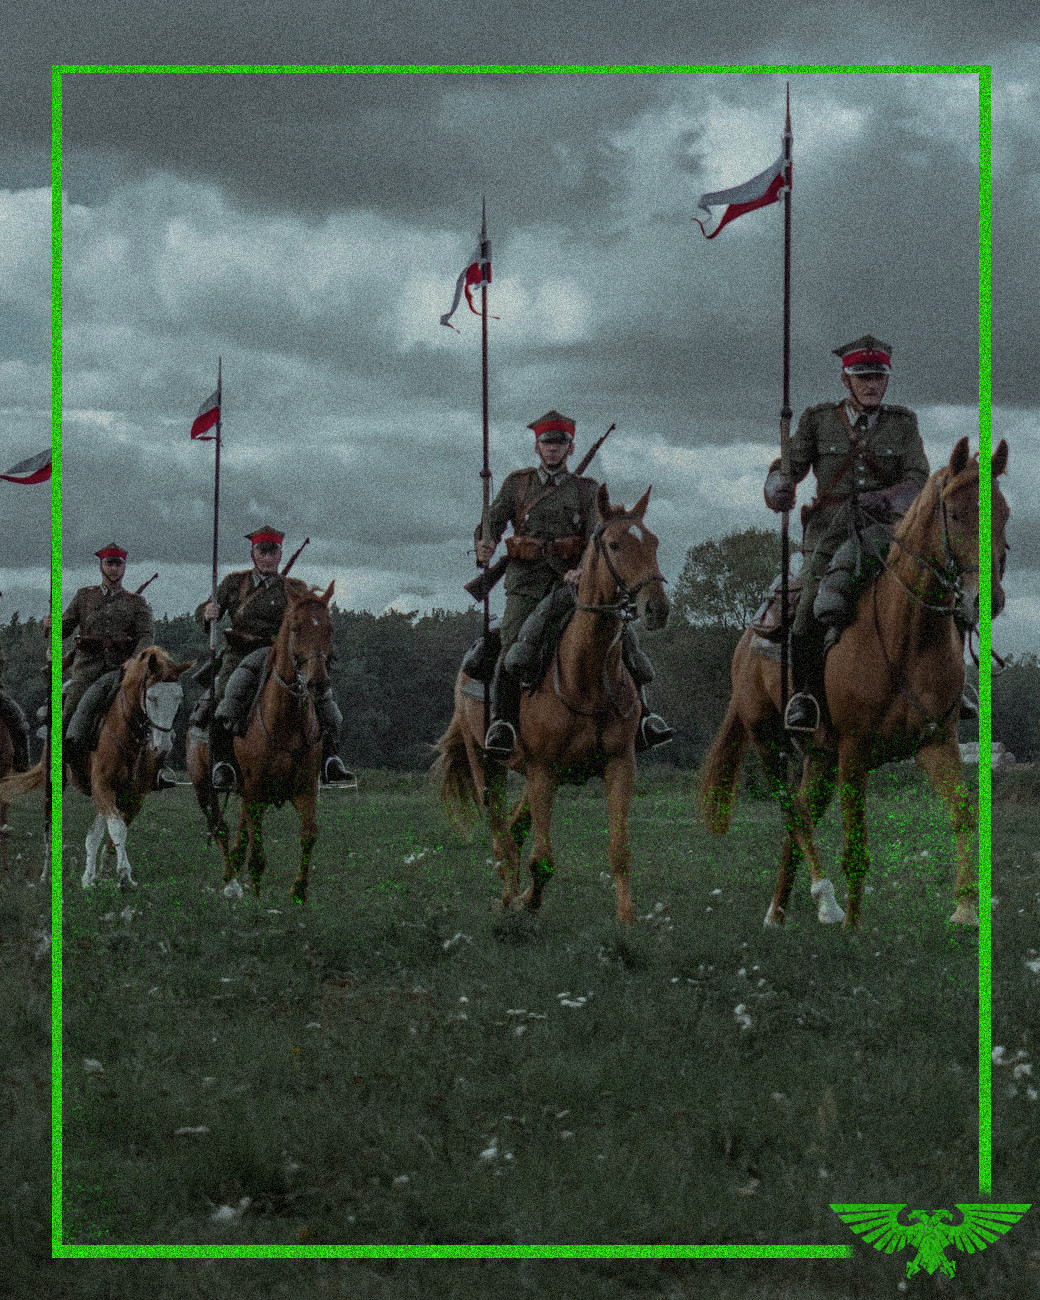
\includegraphics[width = 0.3\textwidth]{patrouille_cav.jpeg}
  \caption{Une patrouille du 3ème de lanciers Messinan avance sur l'agri-monde Palara au cours de l'opération Defiance}
\end{wrapfigure}

La vraie surprise vint de Luzion-null, un monde-forge mineur, que le renseignement de la croisade avait incorrectement identifié comme une simple cible de raids des forces hérétiques. Les études ultérieures de l'ordo hereticus montrèrent qu'il s'agissait sans doute du centre de la corruption dans la région, le culte noir de Baroda s'y étant fermement implanté, et ayant travaillé à développer de nombreuses machines ignobles dans les entrailles des forges et fonderies corrompues. Les troupes impériales n'étaient donc pas prêtes à affronter les hordes de créatures mécaniques infernales que les maîtres des forges lâchèrent sur eux dès leur arrivée. Le tactica imperialis estime de 60\% de la première vague d'assaut fut tué dans les premières heures de débarquement. Une tête de pont réussit à être maintenue sur les hautes-terres de Mika, avant d'être étendue. La situation s'enlisa rapidement face aux stratagèmes des forces hérétiques, et ne put être résolue qu'après des mois d'affrontements stériles grâce à l'intervention de la legio titanique Invicta, dont les armes jetèrent à bas les défenses enterrées de l'ennemi.

Malgré la réussite de tout ses objectifs, cette première phase avait pris plus de temps et d'efforts que prévu, mais les forces impériales ne s'arrêtèrent pas pour consolider leur position, et le maître de guerre lança la seconde étape du plan : l'opération Thunder Strike.
\section{Opération Thunder Strike}
%seconde partie de l'offensive impériale, au cours de laquelle les magos de Baroda sont repoussés, ce qui change grandment la politique des forces du chaos. Route jusqu'à Graal.
Cette seconde phase devait permettre à la croisade de continuer l'offensive jusqu'aux abords de l'abysse de Graal, la cible principale étant le monde de Graal. Un objectif ambitieux, qui, s'il était atteint, mettrai les forces hérétiques sur les talons.

La différence fut immédiate avec Defiance : les forces ennemies pouvaient menèrent plusieurs contre-offensives vicieuses, comme sur Anoter Prime, prise en quelques semaines par les forces impériales, qui durent ensuite défendre la planète pendant près de deux ans sous les assauts de renforts de l'ennemi, au milieu des vents de cendre et des cheminées toxiques.

Les premières estimations du tactica tablaient sur trois à cinq ans de conflit pour arriver au bord de l'abysse de Graal, ce qui permettrait de monter des opérations offensives contre Baroda par la suite. Ces estimations furent par la suite repoussées 13 fois, à mesure que des obstacles de plus en plus importants se trouvèrent face à la croisade, et que des contre-offensives ennemies durent être repoussées. 

\begin{wrapfigure}{r}{0.3\textwidth}
  \centering
  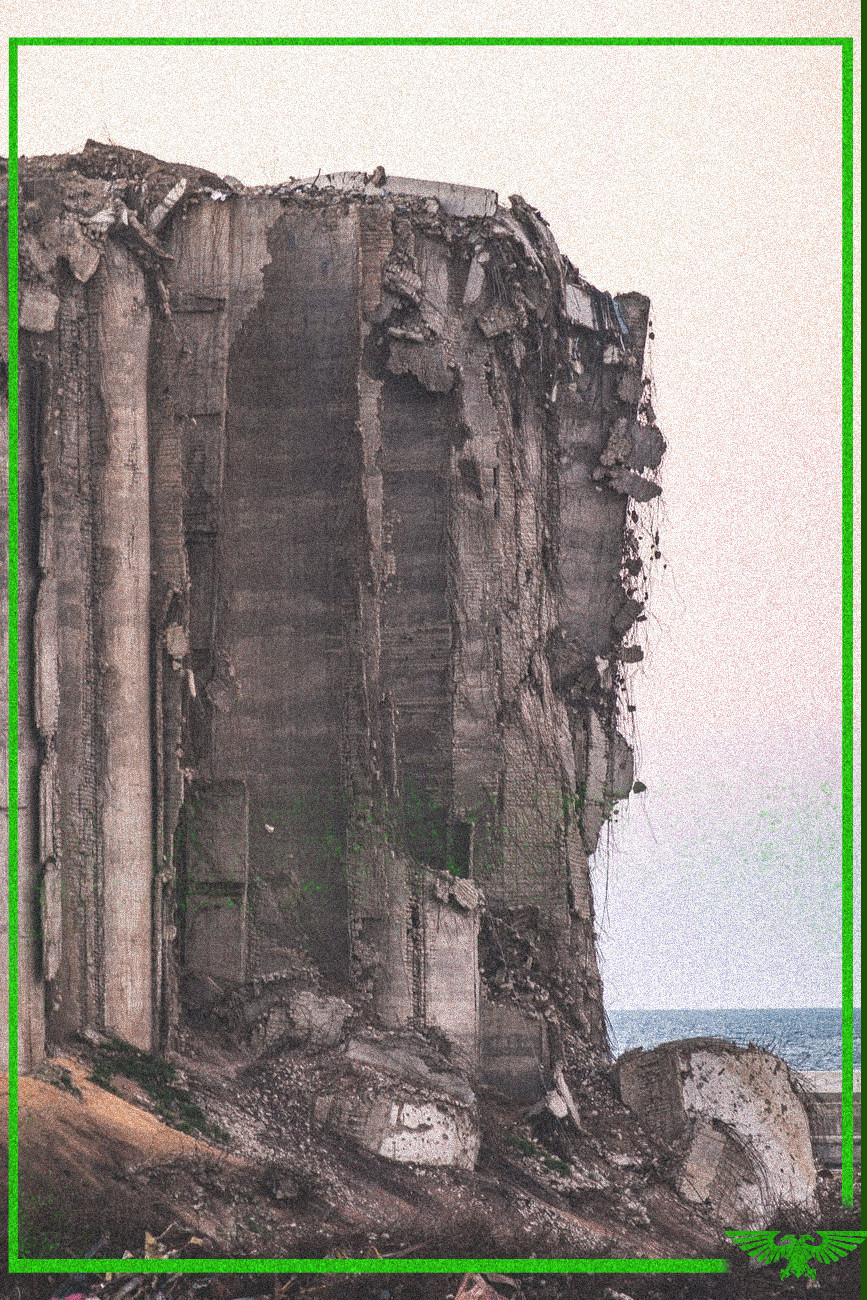
\includegraphics[width = 0.3\textwidth]{ruines 1.jpeg}
  \caption{Les ruines des défenses de la forteresse d'Ankolm, brisée par les sapeurs du 30ème morachéen}
\end{wrapfigure}

A ce stade de la croisade, les troupes impériales avaient une bonne idée de leur adversaire. Le coeur des détachement de l'ennemi était systématiquement une force corrompue du mechanicus, disposant de nombreux engins de morts aussi corrompus que dangereux. Certains modèles communs furent identifiés, mais les vétérans apprirent aussi que beaucoup de ces engins étaient autant des créatures vivantes, capables d'adaptation, que de froides machines à tuer. En plus des sombres constructions des magisters de Baroda, de nombreux hérétiques se battaient également pour l'ennemi, souvent dans un rôle auxiliaire : des renégats de toutes sortes, quelques bandes de guerre du chaos, peut-être issues de l'oeil de la terreur, et des hordes d'esclaves techno-modifiés.



Malgré les difficultés, les forces impériales réussirent à maintenir leur élan au travers des lignes défensives successives de l'ennemi, jusqu'à arriver devant Graal en 859M41, après 8 ans de conflit. Le siège planétaire dura deux années supplémentaires, les troupes impériales subissant une contre-offensive majeure de l'archi-Ordinante Mocian. Celle-ci espérait sans doute décapiter le commandement de la croisade lors de cette campagne. Les lignes de fronts s'étendaient autant sur les nombreuses îles volcaniques de la planète que sur les nombreuses stations spatiales du système. La bataille pour Graal bascula grâce à une percée du 30ème d'infanterie Morachéenne, qui réussit après trois mois d'efforts à faire tomber un des bastions de l'île-forteresse d'Ankolm. Cela permit ensuite à un contingent de kasrkins cadiens de mener un assaut au coeur du dispositif défensif, et d'abattre Mocian après une fusillade de 2 heures avec ses gardes démoniaques. Avec la mort de l'archi-ordinante, les défenses de Graal perdirent en vivacité, chaque magister ou ordinant ne contrôlant plus que ses propres troupes, certains fuyant au plus vite la planète pour éviter son juste châtiment aux mains des forces impériales.
\section{Contre-offensive sur le  \front}
%Nouvelle menace grandissante sous la forme de troupes mieux préparées que celles du darkmech : des troupes relativement disciplinées, toujours armées par Baroda.
%Grande menace pour la croisade
Alors que les forces impériales devaient renforcer leurs positions pour préparer la suite des opérations, et notamment un potentiel assaut sur Baroda, les forces de l'ennemi subissaient de grands changements : nombre des principaux Ordinants étaient morts ou se terraient loin des troupes impériales, ce qui amena plusieurs de leurs lieutenants à renforcer leur propre position.

Un second front fut ouvert vers le regroupement Cyclopéen, afin de sécuriser les flancs de la croisade, s'enfonçant rapidement dans les rangs désorganisés des hérétiques. Toutefois, après quelques mois d'avancées, les forces impériales commencèrent à entendre un nouveau nom, traduisant une nouvelle puissance ennemie : le Praedicator Sirand. Au départ un simple nom sur les briefing de renseignement, rapidement la source de tous les problèmes de la croisade.

Le tactica imperialis a pu déterminer qu'il s'agissait d'un seigneur de guerre de Dark Haven, un ancien monde-chevalier abandonné depuis longtemps par les hauts seigneurs de Terra. Ce seigneur de guerre a repris le contrôle brutal des forces ennemies dans toute la région. Pour cela, il dispose de deux outils principaux : le premier est composé de ses fer-liés, un groupe renégat organisé selon les méthodes des hommes d'armes des maisons de chevaliers. Chacun des 'hommes' qui sert dans les rangs des fers-liés a juré fidélité au praedicator et aux dieux noirs, créant une force bien plus efficace que les hordes de cultistes rendus fous que les croisés avaient l'habitude d'affronter, ou que les machines dirigées par des esprits bestiaux et maléfiques. Son second outil principal est composé des anciens chevaliers de Dark Haven : plusieurs de ces marcheurs de combat semblent toujours opérationnels, et leur dangerosité n'est plus à démontrer.

Les fer-liés opèrent comme un sombre reflet de la garde impériale, avec une organisation militaire rigoureuse et une volonté certaine de détruire l'ennemi. Ils sont divisés en ost (équivalents à un régiment de la garde), puis en bataillons, compagnies.... Ils disposent de leurs propres véhicules, en plus de ceux des autres forces hérétiques, qui leurs servent d'auxiliaires. En particulier, des xenos connus sous le nom de Veers sont fréquemment employés comme infiltrateurs par les fers-liés, même si les liens entre ces deux groupes ne sont pas encore clairs. Pour plus de détails, voir [REDACTED BY ORDER OF THE INQUISITION]. Dans tous les cas, les fer-liés ne devraient pas être sous-estimés par les forces impériales, notamment le sens tactique de leurs officiers n'est pas à négliger.

La supériorité du Praedicator sur les autres seigneurs du chaos de la région se traduit en premier lieu par les serments d'allégeance que ceux-ci ont dû lui faire : même les ordinants de Baroda ont plié le genou, et font maintenant parti de ses 'hérauts', ses lieutenants les plus efficaces. Plus directement pour les forces impériales, les fer-liés ont dirigé une violente série de contre-attaques contre le \front . Prises par surprise par des assauts disciplinés et bien maîtrisés, le \front menace maintenant de s'effondrer. Cela a été renforcé par plusieurs insurrections manigancées par certains des hérauts les plus subtils sur certains de leurs anciens mondes et jusqu'au coeur du sous-secteur Maw.

Aujourd'hui, le seigneur général militant Kalbridge dirige le \front , et a comme priorité absolue la stabilisation de sa ligne et de ses arrières, avant que toute avancée ne puisse se faire. Le maître de guerre de son côté, enrage de ne pas pouvoir aller terminer les ordinant dans leur forteresse de Baroda, mais lance des offensives pour préparer une avancée dans cette direction dès que ses lignes arrières seront plus sûres.
\chapter{Histoire de \zone}
\zone est un monde-ruche proche de Port-Maw, qui a vu son importance grandir rapidement au cours de la croisade : ses productions d'armes et de matériaux sont en effet une source majeure d'approvisionnement pour les troupes engagées sur les différents fronts. Il s'agit depuis longtemps d'un monde stratégique pour l'approvisionnement des troupes dans la région de la porte cadienne, et la situation de la région n'a fait qu'augmenter cette importance.

Les cinq ruches principales coopèrent sur certains points, mais restent des rivales économiques importantes. Avec le temps, certaines spécialités sont toutefois apparues. La capitale planétaire est la ruche Solus, la plus grande de toutes, avec près de 5 milliards d'âmes servant l'empereur dans ses fonderies et diverses industries. La ruche Aventus fournit de nombreux mondes en carburant, en huiles industrielles ainsi qu'en produits chimiques divers; ses alentours sont aussi la région la plus lourdement polluée de la planète. La ruche Idénis était à l'origine une colonie pénale de Solus, et se situe à une relative proximité de sa génitrice. Elle fournit généralement en matières première les autres ruches de la planète. La ruche Austris est au bord de l'océan, et produit de nombreux types de rations militaires ou civiles, ainsi que les millions de kilomètres de rouleaux de papiers nécessaire au bon fonctionnement de l'administratum. Enfin, la ruche Nessus est partiellement souterraine, étant bâtie à l'origine dans une immense crevasse dans l'hémisphère sud de la planète.

Hors des ruches, la majeure partie de la planète est désertique, et l'a toujours été, même avant que la pollution des industries ne soit aussi présente. Les vents sont souvent violents, et déclenchent très régulièrement de redoutables tempêtes de sable, contre lesquelles toutes les ruches disposent de barrières ou de boucliers pour se sceller face aux éléments. Il existe également de nombreuse communautés hors des ruches : des marchands nomades faisant le relai entre les ruches majeures à des villes suffisamment importantes pour disposer de leurs propres défenses environnementales. Au niveau politique, toutes ces communautés sont toutefois subordonnées aux maisons majeures ou mineures des ruches.

La gouverneure planétaire est la dirigeante de la ruche Solus, Dame Merity Chiron, de la maison Chiron. Elle dirige les efforts de sa ruche et s'assure que les autres participent convenablement à la dîme planétaire depuis presque soixante-dix ans, un pouvoir qu'elle ne partage avec personne, même si les héritiers présomptifs sont relativement nombreux.
\section{Au début du millénaire}
Les ruches de \zone ont moins été touchées par le déclin du secteur que les planètes voisines, leur production industrielle étant considérée par l'Imperium comme étant de première importance : du carburant, des cellules énergétiques, ainsi que de nombreux autres articles utilisés par différentes organisations impériales, en particulier l'astra militarum.

Cela signifie que les autorités planétaires disposaient également de contact plus fréquents et importants avec l'administration du secteur, et bénéficiaient d'une bien meilleure protection de la part de la flotte Obscurus, qui défend son bastion de Port Maw. Cela a permit de maintenir la planète dans une relative sécurité et prospérité. 
\section{La croisade \croisade}
La \croisade a lors de ses phases d'ouverture été une aubaine pour \zone : les besoins des forces impériales dans la région ayant grandement augmenté, les exportations des ruches ont gagné en valeur, ce qui a permis également de développer de nouvelles fonderies, usines et installations industrielles diverses. 

Plusieurs régiments ont été levés parmi les Forces de Défense Planétaires, afin de renforcer les effectifs de l'Astra Militarum. Les FDP ont malgré cela pu se renforcer en matière d'équipement en profitant de l'afflux de crédits sur la planète. 

Les nouveaux régiments sont composés de 5 régiments d'infanterie de ligne, issus des forces privées des différentes maisons nobles, 2 régiments de troupes légères, avec des volontaires venus d'hors des ruches, et d'un régiment d'artillerie, fierté de la ruche Nessus, qui a fournit la totalité des pièces et de leurs servants, suite à un accord avec le méchanicus pour disposer des plans de constructions des canons trembleterre. La plupart ont été engagé avec succès sur les différents fronts de la croisade, gagnant plusieurs citations et honneurs de bataille face aux forces du chaos. Une nouvelle fondation était d'ailleurs envisagée, pour lever une nouvelle série de régiments.
\section{La nuit de sang}
Toutefois, dans les bas-fonds des ruches, les forces du chaos murmuraient à l'oreille des mécontents et des marginalisés. 

Dans un premier temps, les habitants des sous-ruches parlèrent de disparitions, de créatures plus dangereuses qu'à l'accoutumée qui rôdaient dans les ombres et les tunnels oubliés. Certains contremaîtres notèrent également que leurs ouvriers semblaient se retrouver plus fréquemment hors de leurs usines.

Avec le temps, l'adeptus arbites nota également une hausse de la désobéissance civile : des groupes d'ouvriers commençaient à protester contre les nouveaux horaires de travail ou les réorganisations rendues nécessaire par les besoins de la croisade. Différentes protestations furent brisées dans le sang, et oubliées par la suite.

\begin{wrapfigure}{l}{0.3\textwidth}
  \centering
  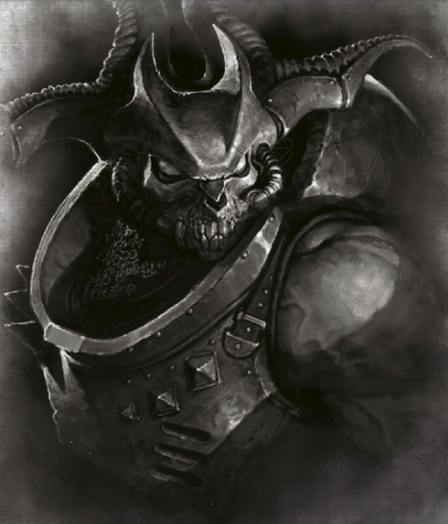
\includegraphics[width = 0.3\textwidth]{chaos 1.png}
  \caption{Image d'un des hérétiques ayant mené l'assaut contre la spire de la ruche Aventus}
\end{wrapfigure}

Pendant ce temps, de petits groupes discrets commençaient à se former, souvent pour protester contre l'oppression de plus en plus forte par les autorités impériales. Ces groupes profitèrent des griefs de beaucoup contre les maisons nobles, mais aussi contre leurs usines, puis, après quelques temps, contre la botte de fer du système impérial.

Peu à peu, les sentiments propagés par ces groupes se firent plus hostiles à l'Imperium. Certains furent découverts, et brutalement exécutés par l'arbites. Les autres continuèrent à propager leur poison : des groupes de mécontents se rassemblèrent dans des bâtiments abandonnés,et proposèrent de l'aide à leurs frères ouvriers. Petit à petit, une part de plus en plus grande des ouvriers des ruches, et surtout, des habitants des sous-ruches, commença à entendre ce discours anti-impérial, et à le propager.

Tout ceci pris fin avec la nuit de sang, en 102.863M41. Il apparut alors à l'inquisition autant qu'à l'arbites que les nombreux groupes étaient coordonnés. En effet, alors qu'un message radio codé était diffusé sur toutes les fréquences, des insurrections armées commencèrent sur toute la surface de la planète.

La ruche Aventus tomba dès la première nuit, les ouvriers des fonderies massacrant rapidement les contremaîtres avant de ravager les maisons nobles de la spire. En l'espace de quelques jours, les dernières poches de résistance impériale avaient été anéanties ou avaient été abandonnées par leurs défenseurs.

Nessus résista plus longtemps, les quatre régiments des FDP ayant été globalement épargnés par les désertions réussirent à tenir le fort Garro et l'astroport adjacent pendant plusieurs semaines, gagnant le temps d'évacuer plusieurs dizaine de milliers de ruchards. D'autres positions furent tenues pendant un temps par les forces impériales, avant de céder sous la pression des assauts fanatiques des forces du chaos.

A Idenis, les milices minières réussirent à tenir les plus grandes installations, aidées par plusieurs groupes improvisés d'ouvriers loyaux à l'Imperium. Après plusieurs semaines de combat et l'intervention d'un régiment de FDP, la plupart des insurgés furent tués ou rejetés dans le désert hors de la ruche, même si des attaques et infiltrations restent fréquentes dans toute la ruche.

Austris fut le théâtre de violents combats, les insurgés n'ayant pas autant réussi à se coordonner qu'ailleurs pour frapper toutes leurs cibles. En particulier, le maréchal Kowle de la maison Kowle échappa de peu à une tentative d'assassinat, et pu diriger d'une main de fer les défenses impériales. Après plusieurs semaines de combat, les forces insurgées et impériales n'avaient pas encore réussit à surpasser leur opposant, même si un équipement supérieur et le commandement du maréchal permirent aux impériaux de regagner du terrain perdu.

Solus fut également le théâtre de féroces affrontements. Au moins deux maisons mineures déclarèrent leur trahison en ravageant la chambre du conseil. A la fin de la première journée, plusieurs maisons nobles avaient été anéanties, et environ 75\% de la ruche était aux mains des insurgés. Les forces de la maison Chiron tenaient encore une partie de leurs cantonnements, la forteresse inquisitoriale et principal bastion de l'adeptus arbites avaient réussi de justesse à repousser une horde d'assaillants fanatisés, et plusieurs régiments des FDP toujours loyaux avaient gagné suffisamment de temps pour se mobiliser et commencèrent à former une défense cohérente. Alors que les navires de guerre impériaux arrivaient en orbite, la position impériale dans Solus était toujours précaire, avec les installations de la maison Chiron toujours assiégées par l'ennemi et isolées régulièrement des autres défenseurs. Le commandement des forces de la maison Chiron et des FDP est enrte les mains du général Nathaniel Chiron, un petit-fils de la gouverneure. Cette dernière a été évacuée vers la ruche Idenis, qui reste entre les mains impériales.



Malgré les efforts des insurgés, un message astropathique avait pu être envoyé à l'imperium pour informer de la situation critique, et au regard de l'importance de \zone , un groupe de renfort fut rapidement mis sur pied pour intervenir, avec certaines des troupes en transit près de ce nouveau front. Il fallut deux mois pour rassembler et faire transiter ces troupes pour intervenir. 
Pendant ce temps, il apparu que la rébellion était sans doute organisée depuis Aventus, dirigée par le magister Kycius, un des hérauts du Praedicator, dont la voix se répandit rapidement sur toutes les fréquences radios. Les forces hérétiques s'organisèrent rapidement pour essayer d'écraser les bastions impériaux, en essayant de faire transiter des troupes d'une ruche à l'autre. En particulier, des groupes venus de Solus avancèrent avec la ruche Idenis, des combats éclatant dans les dunes de sable pollué.
\chapter{Forces impériales}
En plus des troupes loyales à l'imperium au sol, un groupe de combat a été improvisé par le commandement de la croisade pour sauvegarder ses lignes d'approvisionnement et sécuriser son flanc. Celui-ci rassemble des forces qui devaient aller sur d'autres lignes de front et ont été déroutées dans l'urgence.


\section{Forces locales}
Si les FDP disposaient de plusieurs régiments au début des combats, leurs effectifs ont été sérieusement entamés par les deux mois de combat. Ils ont appris à se battre efficacement dans les ruines urbaines de leurs ruches respectives. Leur principal soutien furent les troupes des maisons nobles, même si celles-ci étaient plus utilisées pour intimider la concurrence avant le conflit, et étaient de qualité très variable. Ces unités étaient aussi les seuls à disposer de matériel militaire lourd dans le camps impérial, avant l'arrivée du groupe du seigneur militant Artemenes.

A ceci se sont ajoutées différentes unités de miliciens et groupes improvisés, formées par les habitants des ruches et les différentes usines. Les pertes dans ces groupes ont pu être considérables, par manque d'équipement et d'expérience, mais certaines ont pu se montrer redoutable, généralement grâce à une motivation sans faille à protéger leurs famille et leurs ruches de l'ennemi. Ces groupes plus ou moins improvisés forment la majeure partie des effectifs opérationnel pour le combat dans les ruches.

Enfin, quelques troupes inquisitoriales et de l'arbites ont survécu à la première phase insurrectionnelle, malgré des tentatives des rebelles de les éliminer en premier. Ils forment des groupes de petite taille, mais sans doute les mieux équipés de la planète, et parmi les plus aguerris. En témoigne le siège de la forteresse inquisitoriale de Solus, qui dura quatre semaines avant que ses défenseurs ne puissent être relevés.
\section{Astra Militarum}
Le général Artemenes reçu le commandement du groupe d'intervention impérial, étant promu pour l'occasion au rang de seigneur militant. Il s'agit d'un officier issu des troupes d'assaut Zhannites, décoré pour plusieurs commandements dans la région de la porte cadienne. Il est généralement vu comme impétueux, et relativement jeune pour devenir seigneur militant. Cette position inattendue pourrait l'inciter à faire ses preuves, une victoire lui ouvrant de fantastiques perspectives au sein du Militarum.



Comme ses troupes, il bénéficie de l'expérience de la libération de sa planète natale face à une rébellion similaire, écrasée brutalement après des mois de guerre urbaine brutale, terminée par l'intervention d'astartes du chapitre des Imperial Fists. 




Le groupe de combat sous ses ordres contient une quarantaine de régiments de qualité diverse : certains sortent tout juste de réarmement, comme le 11ème grenadiers royaux Atecan, d'autres à l'inverse sont tout récemment formés et devaient rejoindre des zones de guerre secondaires, comme les premières et secondes brigades cuirassées vespasiennes. La force totale dispose d'environ un million et demi de troupes, ainsi que plusieurs centaines de véhicules de types divers.

\begin{wrapfigure}{l}{0.3\textwidth}
  \centering
  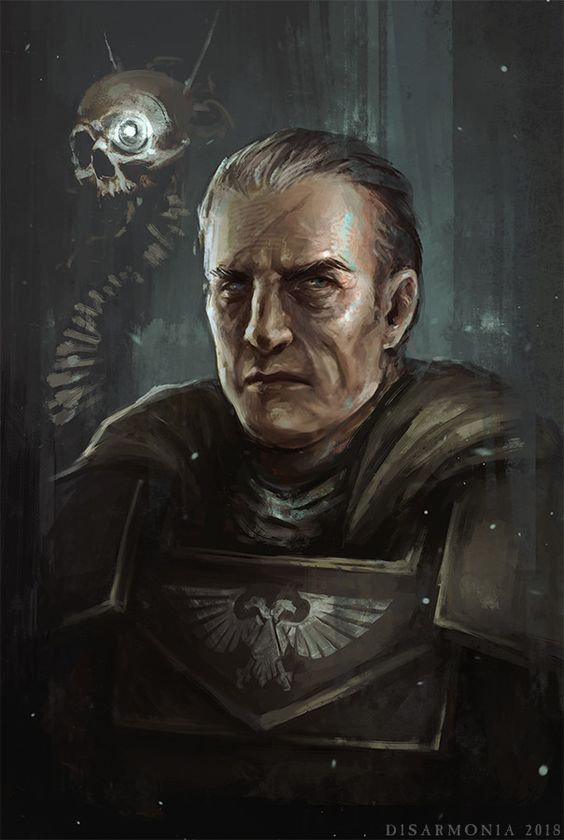
\includegraphics[width = 0.3\textwidth]{officer 1.jpg}
  \caption{Seigneur militant Artemenes, commandant du groupe d'intervention impérial}
\end{wrapfigure}

Le nouveau seigneur général militant va devoir gérer l'arrivée sur une planète principalement hostile, mais aussi les aspects plus politiques de son nouveau rang : il va devoir convaincre les différents éléments de son groupe de combat, appartenant à des organisation impériales très différentes, de travailler ensemble à la destruction des rebelles. En particulier, les forces inquisitoriales ne sont pas sous son autorité, et celles du mechanicus peuvent notoirement nécessiter des négociations.

Le commandement de la croisade estime qu'au vu de l'ampleur de l'insurrection, ce groupe de combat devrait faire l'affaire, ou du moins tenir jusqu'à la mise en place d'un second groupe de renfort si besoin. Les premières projections tactiques suggèrent de sécuriser les ruches encore tenables, puis de lancer un siège de celles tombées complètement aux mains de l'ennemi.

En plus des forces de l'astra militarum, la force d'invasion dispose de 3 escadrons de chasseurs lourds thunderbolt et 2 de bombardiers marauders, afin de gagner la supériorité aérienne face à des forces rebelles mal équipées.

 Au début de la campagne de sécurisation de la planète, le seigneur Artemenes dispose des troupes suivantes à sa disposition :
\begin{center}
\begin{tabular}{c|c}
Type de régiments & effectifs \\ \hline
Troupes de choc cadiennes & 4 régiments\\
Infanterie d'assaut Zhannites & 5 régiments\\ %9
Grenadiers Atecan & 1 régiment \\
Blindés vespasiens & 2 régiments \\
Faucons harakoni & 2 régiments \\
Tirailleurs de Tallarn & 2 régiments \\ %15
Kasrkins & 2 bataillons\\
Skitarii & 3 régiments \\
infanterie de Krieg & 2 régiments\\
chasseurs de Trask & 3 régiments \\
pionners roanniens & 4 régiments \\%24
infanterie Tuleanne  & 2 régiments\\
artillerie Morachéenne & 1 régiment\\
infanterie Morachéenne & 2 régiments \\
reconnaissance lourde de Calanth & 1 régiment\\
infanterie Necromundienne & 1 régiment\\
Infanterie royale de Volpone & 1 régiment
\end{tabular}
\end{center}

\section{Flotte impériale}
Le groupe d'intervention dispose d'une flotte très limitée, basée sur le croiseur \emph{Litany of Glory} et son sister-ship le \emph{Pride of Saint Jus}. En plus de ces deux bâtiments, la flotte dispose de trois escadrons de destroyers et escorte trois transporteurs lourds. Par ailleurs, la flotte dispose de 2 escadrons de chasseurs spatiaux fury pour s'assurer du contrôle spatial.


Cette escadre réduite est sous le commandement du contre-amiral Fenk, un vétéran de longue date. Il sert en effet depuis 125 ans dans la flotte Gothique, ayant gagné ses galons lors des dernières phases de la 12ème croisade noire, puis au cours de nombreuses patrouilles contre les pillards, pirates et renégats de la région. Avec laa croisade, son escadre a reçu plus d'opérations de ligne classique, connaissant le feu en orbite de Luzion-null, et y subissant de lourds dommages. Après un réarmement dans les chantiers de Port Maw, l'escadre vient d'être redirigée pour servir d'escorte à ce groupe d'intervention .

\section{Autres organisations impériales}
En plus de trois régiments de skitarii, le clergé de Mars a fournit l'appui de quelques précieux chevaliers de la maison Krast. Ceux-ci auraient pour la plupart préféré participer à l'affrontement principal contre les forges hérétiques, mais ont accepté de fournir leur appui sur ce front secondaire après d'âpres négociations.

L'inquisition a également fournit un bâtiment léger, équivalent à un destroyer, à l'escadre impériale, disposant de troupes inconnues à son bord. Ils n'ont que peu de contacts avec le reste des forces impériales, dont ils sont indépendants.

Enfin, l'adepta sororitas a envoyé une mission de sœurs de l'ordre de la lance grise, menée par la Palatine Mirya. Les raisons exacts de leur implication sont inconnues, mais leur simple présence augmente le moral des troupes de l'astra militarum engagées à proximité.


\begin{figure}
\begin{center}
\begin{subfigure}[b]{0.3\textwidth}
     \centering 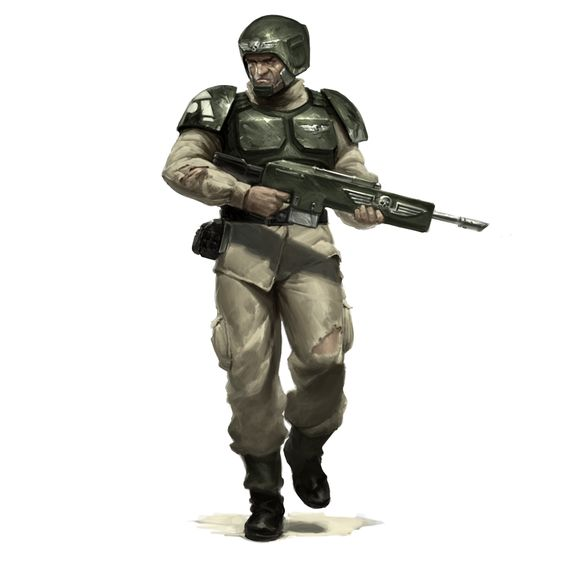
\includegraphics[height = 0.3\textheight]{cadians.jpg}
     \caption{322ème de choc cadien 'fils de Kasr Dun'}
\end{subfigure}
\begin{subfigure}[b]{0.3\textwidth}
     \centering 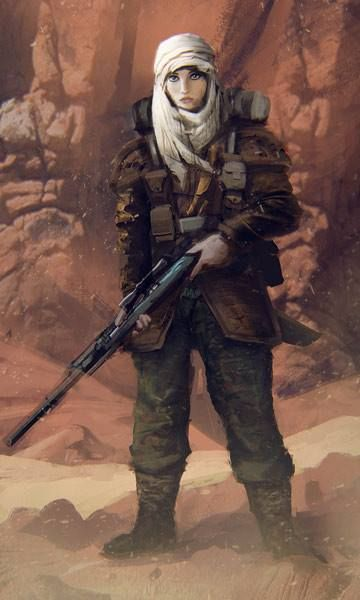
\includegraphics[height = 0.3\textheight]{tallarn.jpg}
     \caption{62ème tirailleur de Tallarn 'sand snakes'}
\end{subfigure}
\begin{subfigure}[b]{0.3\textwidth}
     \centering 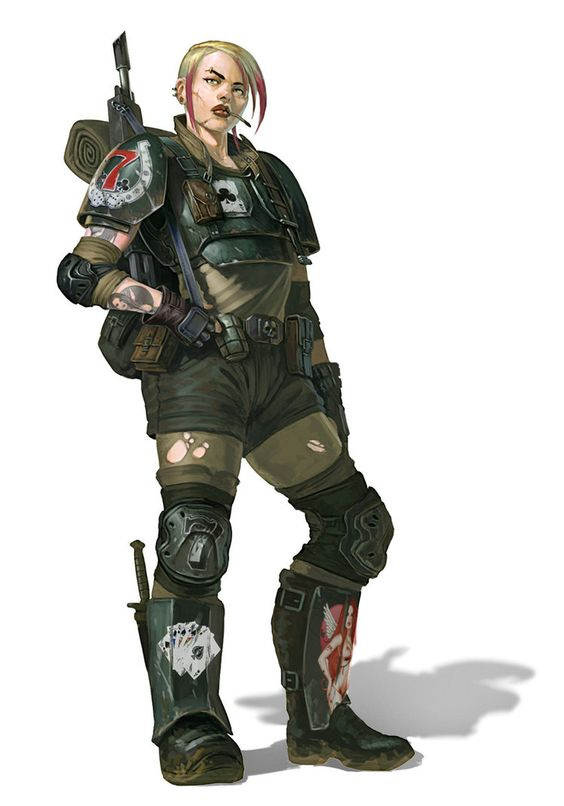
\includegraphics[height = 0.3\textheight]{necromundan.jpg}
     \caption{7ème de Necromunda 'lucky seven'}
\end{subfigure}
\caption{Quelques exemples des régiments du groupe de renforts impériaux}
\end{center}
\end{figure}


\end{document}